\chapter{Ergebnisse und Diskussion}
\label{chap:results}

\section{Darstellung der Daten}
In \tabref{tab:example} werden synthetische Beispieldaten zur Demonstration
von Einheiten, Dezimalstellen und Unsicherheiten gezeigt. Die Unsicherheiten
sind hier als Standardunsicherheiten definiert; ihre Werte sind für dieses
Satzbeispiel frei gewählt.
\begin{table}[htbp]
  \centering
  \caption[Synthetische Beispieldaten]{Synthetische Beispieldaten, keine
    Messwerte. $u_U$ und $u_I$ bezeichnen die zugeordneten
    Standardunsicherheiten von Spannung und Stromstärke.}
  \label{tab:example}
  \begin{tabular}{c S[table-format=1.3] S[table-format=1.3]
                    S[table-format=2.2] S[table-format=1.2]}
    \toprule
    Nr. & {$U/\unit{\volt}$} & {$u_U/\unit{\volt}$}
        & {$I/\unit{\milli\ampere}$} & {$u_I/\unit{\milli\ampere}$} \\
    \midrule
    1 & 1.000 & 0.005 & 10.00 & 0.10 \\
    2 & 2.000 & 0.005 & 20.00 & 0.10 \\
    3 & 3.000 & 0.005 & 30.00 & 0.10 \\
    \bottomrule
  \end{tabular}
\end{table}

In \figref{fig:example-plot} werden dieselben Punkte mit horizontalen und
vertikalen Fehlerbalken dargestellt. Die gestrichelte Modellgerade wird
mit dem vorgegebenen Beispielwert $R=\qty{100}{\ohm}$ gezeichnet; sie ist
keine Regression. Die kleinen Fehlerbalken entsprechen den Beispielwerten
und werden nicht künstlich vergrößert.
\begin{figure}[htbp]
  \centering
  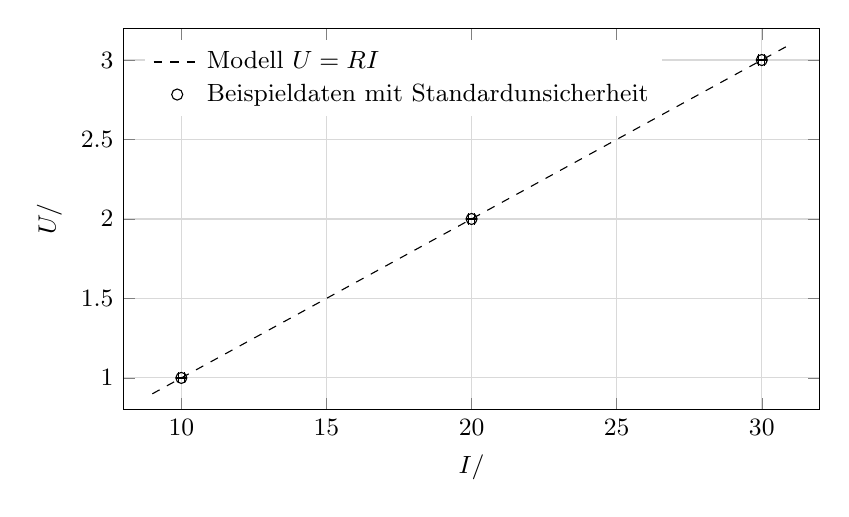
\begin{tikzpicture}
    \begin{axis}[
      width=0.86\linewidth,height=0.53\linewidth,
      xlabel={$I/\unit{\milli\ampere}$},ylabel={$U/\unit{\volt}$},
      xmin=8,xmax=32,ymin=0.8,ymax=3.2,
      xtick={10,15,20,25,30},ytick={1,1.5,2,2.5,3},
      grid=major,grid style={black!15},
      legend pos=north west,legend cell align=left,
      tick label style={font=\small},label style={font=\small},
      legend style={font=\small,draw=none},
    ]
      \addplot[black,dashed,domain=9:31,samples=2] {0.1*x};
      \addlegendentry{Modell $U=RI$}
      \addplot[only marks,mark=o,black,
        error bars/.cd,x dir=both,x explicit,y dir=both,y explicit]
        coordinates {(10,1) +- (0.1,0.005)
                     (20,2) +- (0.1,0.005)
                     (30,3) +- (0.1,0.005)};
      \addlegendentry{Beispieldaten mit Standardunsicherheit}
    \end{axis}
  \end{tikzpicture}
  \caption[Beispieldaten mit Modellgerade]{Synthetische Beispieldaten
    (Kreise mit Fehlerbalken) und vorgegebene Modellgerade (gestrichelt).
    Eigene Darstellung; keine experimentellen Ergebnisse.}
  \label{fig:example-plot}
\end{figure}

\section{Vollständige Beispielrechnung}
Für Zeile 1 in \tabref{tab:example} wird mit \eqnref{eq:ohm} gerechnet:
\begin{equation}
  R = \frac{U}{I}
    = \frac{\qty{1.000}{\volt}}{\qty{10.00e-3}{\ampere}}
    = \qty{100.0}{\ohm}.
  \label{eq:calculation}
\end{equation}
\eqnref{eq:calculation} zeigt Ansatz, eingesetzte Werte und Ergebnis.
Nur für unkorrelierte Eingangsgrößen und bei zulässiger linearer
Unsicherheitsfortpflanzung ergibt sich hier nach \eqnref{eq:uncertainty}
die kombinierte Standardunsicherheit $u_R$ in \unit{\ohm}:
\begin{equation}
  \begin{aligned}
    u_R &= R\sqrt{\left(\frac{u_U}{U}\right)^2
                    +\left(\frac{u_I}{I}\right)^2} \\
        &= \qty{100.0}{\ohm}
           \sqrt{\left(\frac{\qty{0.005}{\volt}}{\qty{1.000}{\volt}}\right)^2
                +\left(\frac{\qty{0.10}{\milli\ampere}}{\qty{10.00}{\milli\ampere}}\right)^2}
         \approx \qty{1.1}{\ohm}.
  \end{aligned}
  \label{eq:uncertainty}
\end{equation}
Damit wird das Beispielergebnis als
$R=\qty{100.0 +- 1.1}{\ohm}$ angegeben. Die Schreibweise bezeichnet hier
die Standardunsicherheit, kein erweitertes Vertrauensintervall.
\offen{Die verwendete Unsicherheitsmethode fachlich belegen und die
Annahmen anhand der realen Messung prüfen.}

\section{Interpretation und Grenzen}
\offen{Reale Ergebnisse mit Erwartungswerten und Literatur vergleichen;
systematische Effekte, Unsicherheiten, Grenzen und mögliche Verbesserungen
diskutieren. Keine Schlussfolgerungen aus den Vorlagendaten übernehmen.}
